\documentclass[a4paper,12pt]{article}

\usepackage[utf8]{inputenc}
\usepackage[T1]{fontenc}
\usepackage[a4paper,total={150mm,240mm}]{geometry}
\usepackage{amsmath}
\usepackage{amsfonts}
\usepackage{amsthm}
\usepackage{amscd}
\usepackage{grffile}
\usepackage{tikz} 
\usepackage{eurosym} 
\usepackage{graphicx}
\usepackage{color}
\usepackage{listings}
\lstset{language=C++, basicstyle=\ttfamily, 
  keywordstyle=\color{black}\bfseries, tabsize=4, stringstyle=\ttfamily,
  commentstyle=\itshape, extendedchars=true, escapeinside={/*@}{@*/}}
\usepackage{paralist}
\usepackage{curves}
\usepackage{calc}
\usepackage{picinpar}
\usepackage{enumerate}
\usepackage{algpseudocode}
\usepackage{bm}
\usepackage{multibib}
\usepackage{hyperref}
\usepackage{textcase}
\usepackage{nicefrac}

\definecolor{listingbg}{gray}{0.95}

\title{DUNE PDELab Tutorial 00 \\ 
Piecewise Linear Finite Elements for the\\
Poisson Equation on Simplices}
\author{Peter Bastian\\
  Universität Heidelberg, \\
  Interdisziplinäres Zentrum für Wissenschaftliches Rechnen\\
  Im Neuenheimer Feld 368, D-69120 Heidelberg\\
  \url{Peter.Bastian@iwr.uni-heidelberg.de}
}
\date{\today}

\begin{document}

\maketitle
\tableofcontents
\clearpage

\section{Introduction}

In this tutorial we solve Poisson's equation with piecewise linear conforming 
finite elements on simplicial elements in one, two and three space dimensions. 
This can be considered as the ``hello world''
example in the numerical solution of partial differential equations which
every software should be able to solve easily (well, there are codes which have
difficulties with triangles). We first provide a short review of the problem and
its finite element solution in order to fix the notation. Then we demonstrate
how this problem is solved using DUNE and PDELab.

\subsection*{Depends On} This tutorial depends on no other tutorials.

\section{Problem Formulation}

\subsection{Strong Formulation}

In this tutorial we consider the {\em Poisson equation}
\begin{subequations}
\begin{align}
-\Delta u & = f \qquad\text{in $\Omega$},\label{eq:1a}\\
u &= g \qquad\text{on $\partial\Omega$},\label{eq:1b}
\end{align}
\end{subequations}
where $\Omega\subset\mathbb{R}^d$ (domains are open and connected sets)
is a given, polyhedral domain (elements with curved
boundaries are possible in DUNE but will not be considered here). 
The problem with homogeneous right hand side $f\equiv 0$ is sometimes called
{\em Laplace equation}. This problem 
is one of the basic equations of mathematical physics which describes gravitational
and electric potential as well as stationary heat or groundwater flow.
Poisson's equation is an instance of an {\em elliptic partial differential equation}.
More about modelling with partial differential equations can be found in \cite{Eriksson,BastianII}.

A function $u\in C^2(\Omega)\cap C^0(\bar\Omega)$ 
(the space of twice continuously differentiable functions in $\Omega$ which are continuous
up to the boundary)
is called a {\em strong solution}
if it satisfies equations \eqref{eq:1a}, \eqref{eq:1b} pointwise. 
Condition \eqref{eq:1b} is called a {\em Dirichlet boundary condition}. Boundary conditions
are necessary to render the solution unique and sometimes one speaks also
of a {\em boundary value problem}.
Formally, one often reduces \eqref{eq:1a}, \eqref{eq:1b}
to a problem with homogeneous Dirichlet boundary conditions $g\equiv 0$ as the
starting point for theoretical considerations. We will deliberately not do this
here as it is also not done in the computer implementation of the method. 

\subsection{Weak Formulation}

Existence, uniqeness and stability of solutions, i.e. well-posedness in the
sense of Hadamard, is easier to prove for so-called weak solutions. As the weak
formulation is also the basis of the finite element method we explain it here.

To start with, suppose $u$ is a strong solution of \eqref{eq:1a}, \eqref{eq:1b} and take 
{\em any } function
$v\in C^1(\Omega)\cap C^0(\bar\Omega)$ with $v=0$ on $\partial\Omega$ then we
have by integration by parts:
\begin{equation*}
\int_\Omega (-\Delta u) v \,dx = 
\int_\Omega \nabla u \cdot \nabla v \,dx= \int_\Omega fv \,dx.
\end{equation*}
Observe that the boundary integral $\int_{\partial\Omega} \nabla u\cdot n v\,dx$ vanishes
due to the fact that $v=0$ on $\partial\Omega$. Loosely speaking $v=0$ is a consequence
of the Dirichlet boundary condition $u=g$ on $\partial\Omega$.

Introducing the abbreviations
\begin{equation}
a(u,v) = \int_\Omega \nabla u \cdot \nabla v \,dx, \qquad l(v) = \int_\Omega fv \,dx
\end{equation}
one can on the other hand ask the question: Is there a class,
more specific a vector space, of functions $V$ with $V_g=\{v\in V : 
\text{$v=g$ on $\partial\Omega$}\}$ and $V_0=\{v\in V : 
\text{$v=0$ on $\partial\Omega$}\}$ such that
the problem
\begin{equation}
u \in V_g :\qquad a(u,v) = l(v) \qquad \forall v\in V_0 \label{eq:weakform}
\end{equation}
has a unique solution. The answer is yes and in particular one can prove the following:
\begin{enumerate}[i)]
\item With $V=H^1(\Omega)$, the Sobolev space of functions with square integrable
weak derivatives, the problem \eqref{eq:weakform} has a unique solution provided
the bilinear form $a : V\times V \to \mathbb{R}$ is continuous and coercive on the 
subspace $V_0\subset V$ and the linear form $l: V \to \mathbb{R}$ is also continuous. 
Coercivity on $V_0$ follows from Friedrich's inequality and for the continuity of the right hand
side functional $f\in L^2(\Omega)$ is a sufficient condition.
\item If in addition $u\in C^2(\Omega)\cap C^0(\bar\Omega)$, then the solution
of \eqref{eq:weakform} and \eqref{eq:1a}, \eqref{eq:1b} coincide.
\end{enumerate}
We call \eqref{eq:weakform} the {\em weak formulation} of \eqref{eq:1a}, \eqref{eq:1b}.
As it has a unique solution under more general conditions than \eqref{eq:1a}, \eqref{eq:1b},
e.g. discontinuous right hand side functions $f$, it can be considered as a generalization
of the problem.

\section{The Finite Element Method}

The (conforming) finite element method, in a nutshell, is based on the weak formulation where
the function space $V$ is replaced by a subspace $V_h\subset V$ 
which is {\em finite dimensional}. Here, the subscript $h$ relates to the dimension of the
function space. One major part of the finite element method is to construct such
so-called {\em finite element spaces}.
Typically, finite element spaces are piecewise polynomial functions.
We consider one particular choice, the space of linear functions on simplicial elements.
There are many text books about the finite element method,
a small selection is
\cite{Eriksson,Ern,Ciarlet,Braess,Brenner,Elman2005,GR,WHElliptisch,RannacherII,BastianII}.

\subsection{Finite Element Mesh}

In order to construct a finite element space a finite element mesh is required.
For simplicity we just consider meshes consisting of $d$-simplices, where a simplex
in $d$ dimensions is the convex hull of $d+1$ points $x_{0},\ldots,x_{d}\in\mathbb{R}^d$
(thus a simplex is, by definition, a closed set of points).

The finite element mesh consists of an ordered set
\begin{equation}
\mathcal{X}_h = \{x_1,\ldots,x_N\}
\end{equation}
of points in $\mathbb{R}^d$ called {\em vertices} and an ordered set 
\begin{equation}
\mathcal{T}_h = \{T_1, \ldots, T_M\}
\end{equation}
of $d$-simplices called {\em elements}.
The elements form a partition of the polygonal domain $\Omega$
\begin{equation}
\bigcup_{T\in \mathcal{T}_h} T = \overline{\Omega}, \quad 
\forall T, T' \in \mathcal{T}_h, T\neq T' : \mathring{T} \cap \mathring{T}' = \emptyset,
\end{equation}
and where each of the vertices $x_{T,0},\ldots,x_{T,d}$  of a $d$-simplex $T\in\mathcal{T}_h$
coincides with a vertex of the set $\mathcal{X}_h$ (and every $x\in\mathcal{X}_h$ is a vertex
of at least one element).

A simplicial mesh is called {\em conforming} if
the intersection of two different elements, $T\cap T'$, is either
empty or a facet (a simplex of lower dimension, i.e. a vertex, edge, face) of {\em both} elements.

The association of the local numbering of vertices within each element 
and the global numbering of vertices in the vertex set is facilitated
via the {\em local to global map} defined by:
\begin{equation}
\forall T\in\mathcal{T}_h, 0\leq i \leq d: g(T,l) = j \Leftrightarrow x_{T,l} = x_{j} .
\end{equation}
The map $g:\mathcal{T}_h\times\{0,\ldots,d\}\to\mathcal{N}$ 
plays also a very important role in the implementation of the finite element method.
Note also that the symbol $g$ is used for the local to global map and the Dirichlet
boundary conditions but it should always be clear from the context which function is meant.

The {\em index set of the vertices} is denoted by $\mathcal{I}_h=\{1,\ldots,N\}$.
It can be partitioned into indices of interior and boundary vertices:
\begin{equation*}
\mathcal{I}_h = \mathcal{I}_h^{int}\cup\mathcal{I}_h^{\partial\Omega},
\quad \mathcal{I}_h^{int} = \{i\in \mathcal{I}_h\,:\, x_i\in\Omega\},
\quad \mathcal{I}_h^{\partial\Omega} = \{i\in \mathcal{I}_h\,:\, x_i\in\partial\Omega\}.
\end{equation*}

In order to illustrate the notation introduced, 
Figure \ref{fig:femesh} shows an example of a conforming finite element
mesh in two space dimensions with its numbering of vertices and elements,
as well as the local to global map.

Finally, by
\begin{equation}
h = \max_{T\in\mathcal{T}_h} \text{diam}(T)
\end{equation}
we denote the {\em mesh size}.

\begin{figure}
\begin{center}
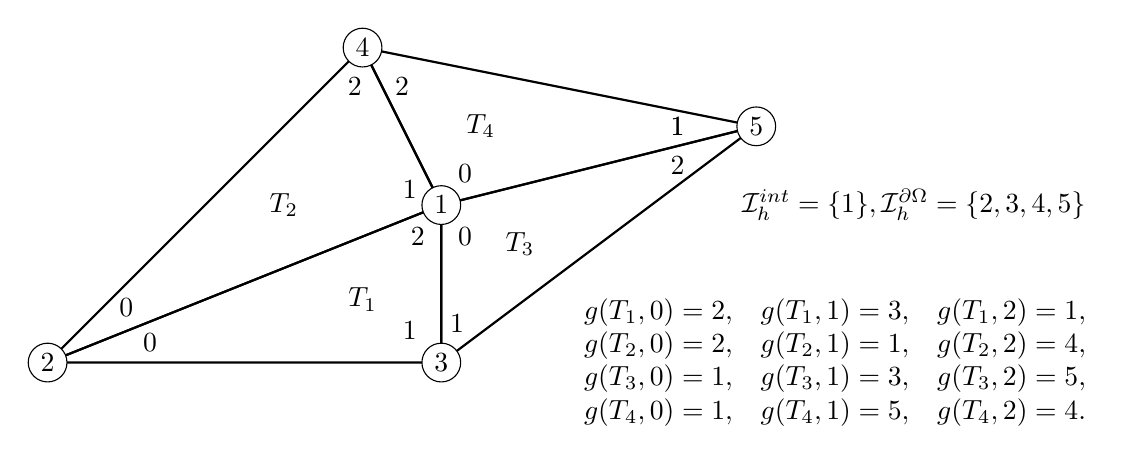
\begin{tikzpicture}[scale=1.0,baseline=(current bounding box.center)]
\draw[thick] (0,0) -- (5,0) -- (5,2) -- cycle;
\draw[thick] (0,0) -- (5,2) -- (4,4) -- cycle;
\draw[thick] (5,0) -- (9,3) -- (5,2) -- cycle;
\draw[thick] (5,2) -- (9,3) -- (4,4) -- cycle;
\node at (4,0.8) {$T_1$};
\node at (3,2) {$T_2$};
\node at (6,1.5) {$T_3$};
\node at (5.5,3) {$T_4$};
\filldraw[fill=white,draw=black] (5,2) circle (7pt) node {$1$};
\filldraw[fill=white,draw=black] (0,0) circle (7pt) node {$2$};
\filldraw[fill=white,draw=black] (5,0) circle (7pt) node {$3$};
\filldraw[fill=white,draw=black] (4,4) circle (7pt) node {$4$};
\filldraw[fill=white,draw=black] (9,3) circle (7pt) node {$5$};
\node at (1.3,0.25) {$0$}; % 2
\node at (1,0.7) {$0$};
\node at (4.6,0.4) {$1$};
\node at (5.2,0.5) {$1$};
\node at (4.7,1.6) {$2$};
\node at (5.3,1.6) {$0$};
\node at (5.3,2.4) {$0$};
\node at (4.6,2.2) {$1$};
\node at (8,2.5) {$2$};
\node at (8,3) {$1$};
\node at (8,3) {$1$};
\node at (3.9,3.5) {$2$};
\node at (4.5,3.5) {$2$};
\node at (10,0) {$%
\begin{array}{lll} 
g(T_1,0) = 2, & g(T_1,1) = 3, & g(T_1,2) = 1, \\
g(T_2,0) = 2, & g(T_2,1) = 1, & g(T_2,2) = 4, \\
g(T_3,0) = 1, & g(T_3,1) = 3, & g(T_3,2) = 5, \\
g(T_4,0) = 1, & g(T_4,1) = 5, & g(T_4,2) = 4.
\end{array}$};
\node at (11,2) {$\mathcal{I}_h^{int}=\{1\}, \mathcal{I}_h^{\partial\Omega}=\{2,3,4,5\}$};
\end{tikzpicture}
\end{center}
\caption{Example of e finite element mesh and the local to global numbering.}
\label{fig:femesh}
\end{figure}

\subsubsection*{Reference Elements and Element Transformation}

The geometry of the mesh elements can be described more easily by
reference elements and an element transformation map. To that end, the
reference $d$-simplex is defined by
\begin{equation*}
\hat T^d = 
\left\{ x\in\mathbb{R}^d \,:\, 0\leq \sum_{i=0}^d (x)_i \leq 1 \wedge \forall i: (x)_i\geq 0 \right \}.
\end{equation*}
The vertices of the reference $d$ simplex are given by
\begin{equation*}
\hat x_0^d = (0,\ldots,0)^T, 
\quad \forall i,j \in \{ 1,\ldots,d\} : (\hat x_i^d)_j = \delta_{i,j}.
\end{equation*}
Figure \ref{fig:refelems} shows the reference elements of dimension 1, 2 and 3
with their numbering of the vertices.

\begin{figure}
\begin{center}
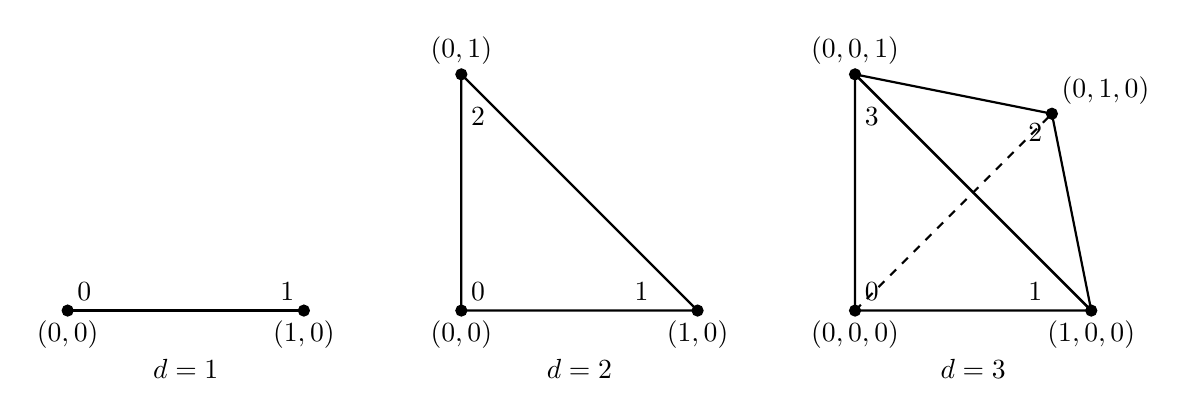
\begin{tikzpicture}[scale=1.0,baseline=(current bounding box.center)]
%d=1
\node[below] at (1.5,-0.5) {$d=1$};
\filldraw (0,0) circle [radius=2pt] node[below] {$(0,0)$}
              (3,0) circle [radius=2pt] node[below] {$(1,0)$};
\draw[thick] (0,0) -- (3,0);
\node[above right] at (0,0) {$0$};
\node[above left] at (3,0) {$1$};
%d=2
\node[below] at (6.5,-0.5) {$d=2$};
\filldraw (5,0) circle [radius=2pt] node[below] {$(0,0)$}
              (8,0) circle [radius=2pt] node[below] {$(1,0)$}
              (5,3) circle [radius=2pt] node[above] {$(0,1)$};
\draw[thick] (5,0) -- (8,0) -- (5,3) -- cycle;
\node[above right] at (5,0) {$0$};
\node[above left] at (7.5,0) {$1$};
\node[below right] at (5,2.7) {$2$};
%d=3
\node[below] at (11.5,-0.5) {$d=3$};
\filldraw (10,0) circle [radius=2pt] node[below] {$(0,0,0)$}
              (13,0) circle [radius=2pt] node[below] {$(1,0,0)$}
              (10,3) circle [radius=2pt] node[above] {$(0,0,1)$}
              (12.5,2.5) circle [radius=2pt] node[above right] {$(0,1,0)$};
\draw[thick] (10,0) -- (13,0) -- (10,3) -- cycle;
\draw[thick] (13,0) -- (12.5,2.5) -- (10,3) -- cycle;
\draw[thick,dashed] (10,0) -- (12.5,2.5);
\node[above right] at (10,0) {$0$};
\node[above left] at (12.5,0) {$1$};
\node[below left] at (12.5,2.5) {$2$};
\node[below right] at (10,2.7) {$3$};
\end{tikzpicture}
\end{center}
\caption{The reference simplices in dimension 1, 2, 3 with vertex positions and
local numbering}
\label{fig:refelems}
\end{figure}

The relation between the reference elements and the elements of the mesh
is provided by the {\em element transformation maps}.
For each element $T\in\mathcal{T}$ there is a map
$$\mu_T : \hat T \to T$$ which maps points of the reference element to the
given element $T$. In an {\em affine} mesh the map $\mu_T$ is affine linear, i.e. it
has the form 
\begin{equation*}
\mu_T(\hat x) = B_T \hat x + a_T
\end{equation*}
for given $d\times d$ matrices $B_T$ and $d$-vectors $a_T$.
Consistency of the local vertex numbering is ensured by the condition
$$\forall i\in\{0,\ldots,d\} : \mu_T(\hat x_i) = x_{T,i}.$$

\subsection{Piecewise Linear Finite Element Functions}

Given a conforming, simplicial and affine finite element mesh in $d$ dimensions we
now can define the space of piecewise linear finite element functions $V_h$.
It is given by
\begin{equation}
V_h(\mathcal{T}_h) = \{ v\in C^0(\overline{\Omega}) \,:\, 
\forall T\in\mathcal{T}_h : v|_T\in\mathbb{P}_1^d\}
\label{eq:Vh}
\end{equation}
where $$\mathbb{P}_1^d = \{ p : \mathbb{R}^d \to \mathbb{R}
\,:\, p(x) = a^Tx+ b, a\in\mathbb{R}^d, b\in\mathbb{R}\}$$
is the vector space of multivariate polynomials of degree one in $\mathbb{R}^d$.
It turns out that the condition of continuity is crucial to ensure that $V_h\subset H^1(\Omega)$.
This definition of the finite element space given above does not refer to a basis.
However, for the practical computations one requires a basis for the
finite element space. Analysis reveals that the dimension of the finite element
space $V_h$ is related to the number of vertices of the mesh:
$$\text{dim} V_h = N = \text{dim} \mathcal{X}_h.$$
Therefore, one may construct a basis $\Phi_h=\{\phi_1,\ldots,\phi_N\}$ of $V_h$ 
where each basis function $\phi_i$ is related to vertex $x_i\in\mathcal{X}_h$ in the following way:
\begin{equation*}
\forall i,j\in\mathcal{I}_h \,:\, \phi_i(x_j) = \delta_{i,j}. 
\end{equation*}
A basis with this property is called a {\em Lagrange basis}.
Exploiting this property of the basis we may define the subspace of
finite element functions satisfying homogeneous Dirichlet boundary conditions
\begin{equation*}
V_{h,0} = \{v\in V_h \,:\, \forall i\in\mathcal{I}_h^{\partial\Omega} : v(x_i)=0\}
\end{equation*}
and the set of finite element functions satisfying the
given boundary conditions \eqref{eq:1b}:
\begin{equation*}
V_{h,g} = \{v\in V_h \,:\, \forall i\in\mathcal{I}_h^{\partial\Omega} : v(x_i)=g(x_i)\}.
\end{equation*}
Note that $V_{h,0}$ is a subspace of $V_h$ and satisfies the homogeneous
boundary data exactly whereas $V_{h,g}$ is {\em not} a subspace (it is an affine space)
and only {\em approximates} the given boundary data by piecewise linear functions.
Twodimensional Lagrange basis functions are illustrated in FIgure \ref{fig:p1basis}.

\begin{figure}
\begin{center}
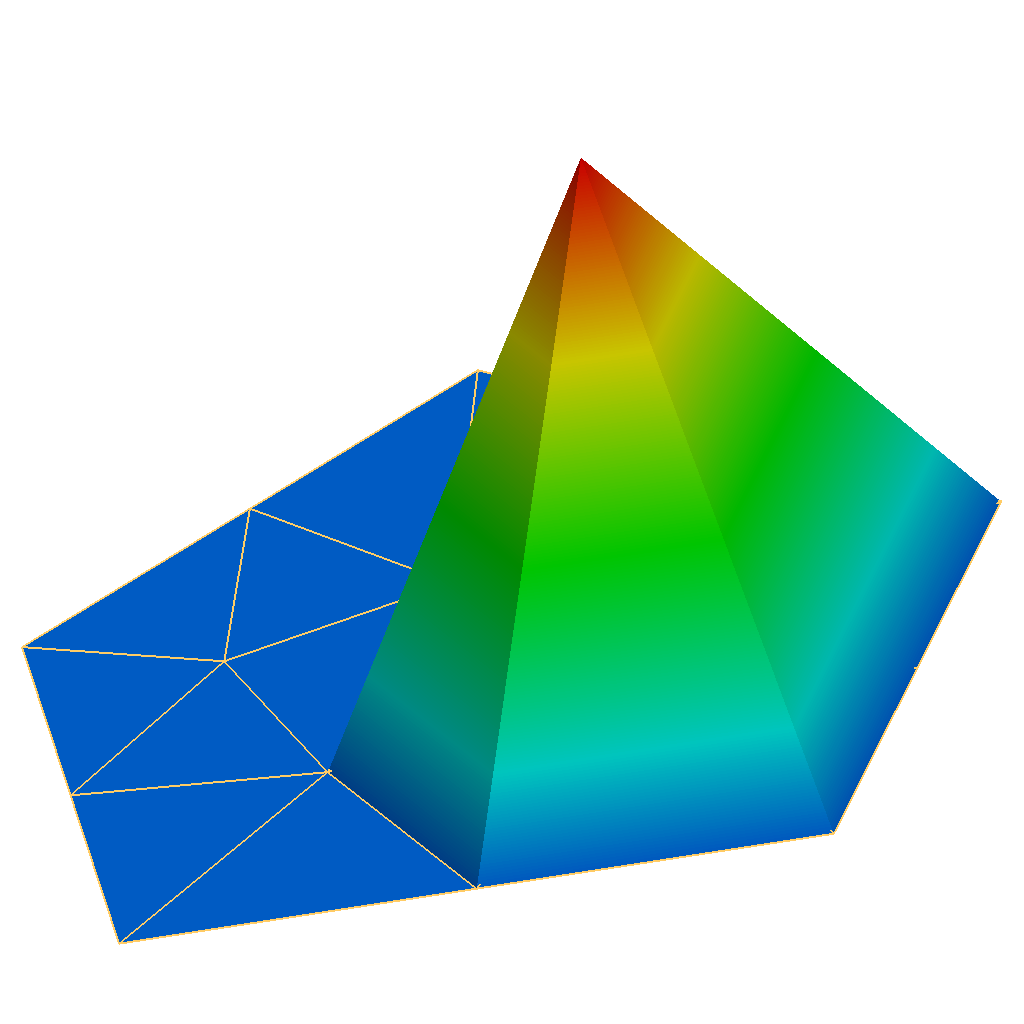
\includegraphics[width=0.4\textwidth]{p1_1}\hspace{0.1\textwidth}
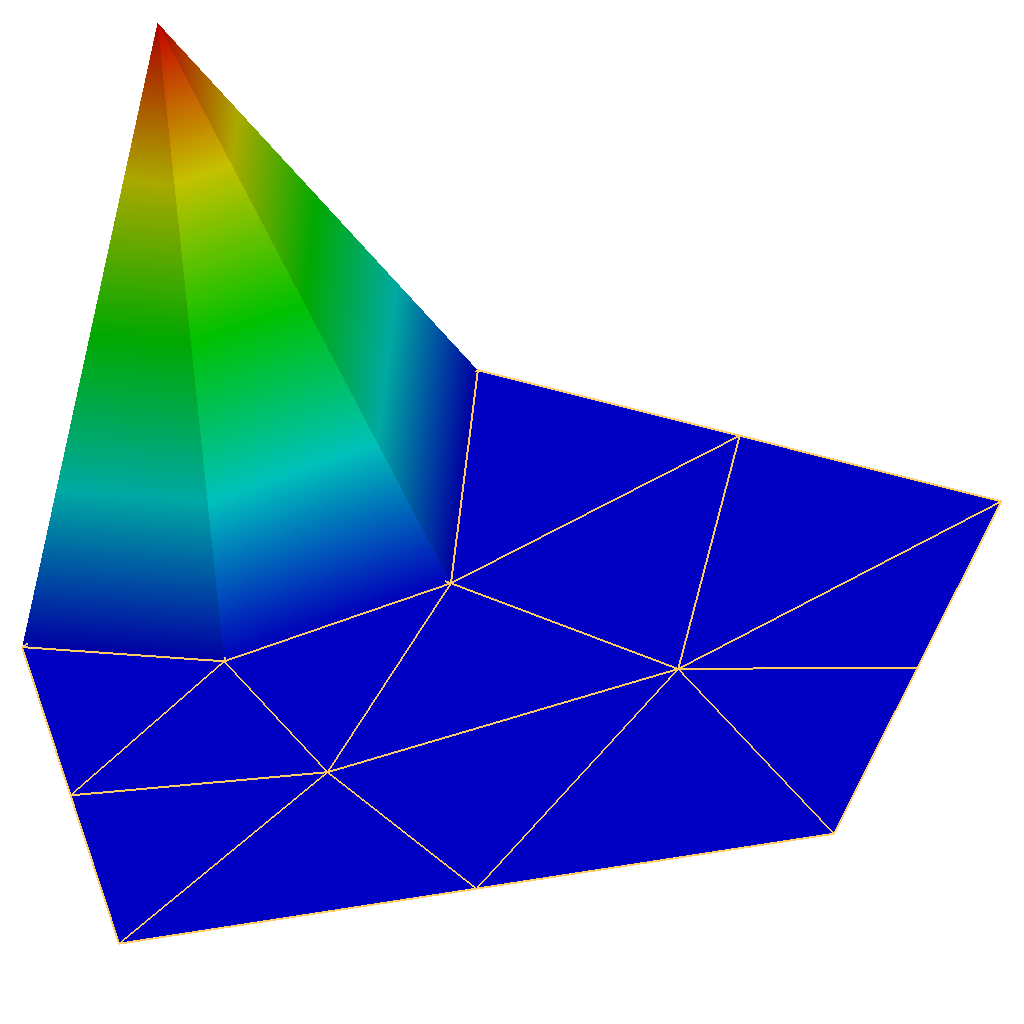
\includegraphics[width=0.4\textwidth]{p1_2}
\end{center}
\caption{Illustration of piecewise linear Lagrange basis functions in 2d. Left one 
corresponds to an interior vertex, right to a boundary vertex.}
\label{fig:p1basis}
\end{figure}

\subsection{Finite Element Solution}

We are now in a position to define and solve the finite element problem.
As pointed out above, the idea is to solve the weak formulation in appropriate
finite-dimensional spaces, i.e.:
\begin{equation*}
u_h\in V_{h,g} : \quad a(u_h,v) = l(v) \quad \forall v\in V_{h,0} .
\label{eq:discrete_weak}
\end{equation*}
Using the Lagrange basis defined above we may expand $u_h\in V_h$ as
\begin{equation*}
u_h = \sum_{j=1}^N (z)_j \phi_j
\end{equation*} 
with coefficient vector $z\in\mathbb{R}^N$. Inserting into the
discrete weak formulation \eqref{eq:discrete_weak} yields:
\begin{align}
a(u_h,v) &= l(v) \quad \forall v\in V_{h,0} &&\text{(discrete weak problem)},\nonumber \\
\Leftrightarrow 
a\left(\sum_{j=1}^N (z)_j \phi_j,\phi_i\right) &= l(\phi_i) \quad \forall i\in \mathcal{I}_h^{int} 
&&\text{(insert basis, linearity)}, \nonumber \\
\Leftrightarrow 
\sum_{j=1}^N (z)_j a\left( \phi_j,\phi_i\right) &= l(\phi_i) \quad \forall i\in \mathcal{I}_h^{int} 
&&\text{(linearity)}. \label{eq:linear1}
\end{align}
The condition $u_h\in V_{h,g}$ can be formulated as a set of equations
\begin{equation}
u_h(x_i) = z_i = g(x_i) \quad\forall i\in\mathcal{I}_h^{\partial\Omega}
\label{eq:linear2}
\end{equation}
which are also linear. Combining the equations \eqref{eq:linear1} and \eqref{eq:linear2}
into a single system of linear equations results in
\begin{equation}
A z = b \label{eq:thesystem}
\end{equation}
where
\begin{equation}
(A)_{i,j} = \left\{\begin{array}{ll}
a(\phi_j,\phi_i) & i\in\mathcal{I}_h^{int}\\
\delta_{i,j} & i\in\mathcal{I}_h^{\partial\Omega}
\end{array}\right., \quad
(b)_{i} = \left\{\begin{array}{ll}
l(\phi_i) & i\in\mathcal{I}_h^{int}\\
g(x_i) & i\in\mathcal{I}_h^{\partial\Omega}
\end{array}\right. .
\label{eq:systemdetail}
\end{equation}
This system may be solved in various ways. The first option are direct solvers
based on some form of the Gaussian elimination technique. However, the matrix $A$
is very sparse as it contains only relatively few nonzero elements per row (3 for $d=1$,
about $7$ for $d=2$ and about $14$ for $d=3$ and Gaussian elimination
may have difficulties to exploit this fact, especially for $d=3$.

Another option is to solve the system iteratively. As the matrix is symmetric and positive
definite there is a variety of methods available which produce, starting from an
initial iterate $z^0$, a convergent sequence $\lim_{k\to\infty} z^k = z$. As a solution
one accepts the first iterate which satisfies the computable criterion
$\|b-Az^k\| < \epsilon \|b-Az^0\|$ for a given reduction factor $\epsilon$.

A very simple (but not very effective) method is {\em Richardson iteration} which is
used to illustrate the concept. It is given by the formula
$$ z^{k+1} = z^{k} + \omega (b-Az^{k}).$$
Algorithmically, this iterative method can be implemented as follows:
\begin{algorithmic}[1]
\State Given $A, b, \epsilon$ and $z$ \Comment{input data}
\State $d = b-Az$ \Comment{compute initial defect}
\State $\tau = \epsilon \|d\|$ \Comment{compute target threshold}
\While{$\|d\|\geq\tau$} \Comment{run until convergence}
\State $z = z + \omega d$ \Comment{update solution}
\State $y = A d$ \Comment{matrix-vector product}
\State $d = d - \omega y$ \Comment{update defect}
\EndWhile
\end{algorithmic}
It can be observed that the matrix $A$ is only involved in matrix-vector
products in lines 2 and 6, an observation that is true for most iterative
solvers. This operation can effectively take into account the sparsity structure
of the matrix and only computations for non-zero elements are necessary.
Thus, one iteration can be implemented with effort $O(N)$. 
The other major factor in the total work is then the number
of iterations needed to achieve the convergence criterion. To keep this
number to an acceptable level effective preconditioners are required.
We do ignore any discussions on effective preconditioners here but they may require 
a major portion of the total work.

Matrix-vector products $y=Az$, require between one and three memory accessess for two
floating point operations as there is never any reuse of the matrix elements.
The exact number depends on the cache reuse of $x$ and $y$ (this is true for
dense and sparse matrices). This fact leads to a very low floating point performance
on modern processors which are much better at computations than at memory access.
A possibility out of this dilemma is to perform the matrix-vector  product in a
{\em matrix-free} fashion, i.e. to recompute the matrix elements while performing
the matrix-vector product instead of storing them. This may lead to a faster 
execution of this operation, especially for certain high-order elements.
Let us consider the matrix-free execution of the matrix-vector product, 
better called {\em operator evaluation}, in more detail.
For $i\in\mathcal{I}_h^{int}$ we get
\begin{equation}
(Az)_i = \sum_{j=1}^N (A)_{i,j} (z)_j = \sum_{j=1}^N a(\phi_j,\phi_i) (z)_j = 
 a\left(\sum_{j=1}^N (z)_j\phi_j,\phi_i\right) = a(u_h,\phi_i) 
\label{eq:opeval}
\end{equation}
where $u_h$ is the finite element function with the coefficients $z$. On the other
hand, for $i\in\mathcal{I}_h^{\partial\Omega}$ we have
\begin{equation*}
(Az)_i = \sum_{j=1}^N \delta_{i,j} (z)_j = (z)_i .
\end{equation*}
We may summarize the typical steps needed to solve the 
finite element problem as follows:
\begin{enumerate}[1)]
\item Assembling the matrix $A$. This mainly involves the computation of the matrix
elements $a(\phi_j,\phi_i)$ and storing them in an appropriate data structure.
\item Assembling the right hand side vector $b$. This mainly involves evaluations of
the right hand side functional $l(\phi_i)$.
\item Perform a matrix free operator evaluation $y=Az$. This involves evaluations
of $a(u_h,\phi_i)$ for all test functions $\phi_i$ and a given function $u_h$.
\end{enumerate}

\subsection{Implementation of the Solution Steps}\label{subs:impl}

We now consider the three operations outlined in the previous section
in more detail. The efficient implementation of these operations involves
the reference elements and the element transformation as part of the following
tools:
\begin{enumerate}[Tool 1)]
\item Transformation formula for integrals. For $T\in\mathcal{T}_h$ we have
\begin{equation*}
\int_T y(x)\,dx = \int_{\hat T} y(\mu_T(\hat x)) \det B_T \,dx .
\end{equation*}
\item Quadrature formula. The midpoint rule reads
\begin{equation*}
\int_{\hat T} q(\hat x) \,dx = q(\hat S_d) w_d
\end{equation*}
where $\hat S_d$ is the center of mass of the reference simplex $\hat T^d$
and $w_d$ is the volume of $\hat T^d$. This quadrature formula is exact for linear
functions.
\item Shape functions. On the reference simplex the linear Lagrange
basis functions are $\hat\phi_i(\hat x) = (\hat x)_i$ for $i>0$ and 
$\hat\phi_0(\hat x) = 1-\sum_{i=1}^d (\hat x)_i$. The basis functions
on a general element $T$ can then be defined via transformation
\begin{equation*}
\phi_{T,i}(\mu_T(\hat x)) = \hat\phi_i(\hat x) .
\end{equation*}
This construction principle can be extend to any function defined on the
reference element. Given $\hat w(\hat x)$ then 
\begin{equation}
w(\mu_T(\hat x))=\hat w(\hat x)
\label{eq:tranformedfunction}
\end{equation}
is the corresponding function on the general element.
\item Computation of gradients. The construction via the reference element
is particularly useful when computing gradients of functions on the general element.
applying the chain rule to \eqref{eq:tranformedfunction} gives
\begin{equation*}
B_T^T \nabla w(\mu_T(\hat x)) = \hat\nabla \hat w(\hat x) \quad\Leftrightarrow\quad
\nabla w(\mu_T(\hat x)) = B_T^{-T}\hat\nabla \hat w(\hat x) .
\end{equation*}
Gradients can be computed by computing gradients on the reference element
and multiplying them with $B_T^{-T}$.
\end{enumerate}
Note that all these tools can be extended to higher order basis functions
and more general element transformations.

\subsubsection*{Assembly of the Right Hand Side}

We start with the assembly of the right hand side vector $b$
defined in equation \eqref{eq:systemdetail}. Since there are typically much more 
interior vertices than boundary vertices we may first compute $(b)_i = l(\phi_i)$
for {\em all} $i\in\mathcal{I}_h$ and then overwrite the entries on the boundary
with $(b)_i = g(x_i)$. Moreover, when considering the global index $i$
only the pairs in the set
$$C(i) = \{(T,m)\in\mathcal{T}_h\times\{0,\ldots,d\} \,:\, g(T,m)=i\}$$
contribute to the computation which can carried out in the following way:
\begin{align*}
(b)_i &= l(\phi_i) = \int_\Omega f \phi_i\,dx &&\text{(definition)} \\
&= \sum_{T\in\mathcal{T}_h} \int_T f \phi_i\,dx &&\text{(use mesh)} \\
&= \sum_{(T,m)\in C(i)} \int_{\hat T} f(\mu_T(\hat x)) \hat\phi_m(\hat x) \det B_T\,dx 
&&\text{(localize)} \\
&= \sum_{(T,m)\in C(i)} 
f(\mu_T(\hat S_d)) \hat\phi_m(\hat S_d) \det B_T w_d \, + \text{error}. &&\text{(employ quadrature)} 
\end{align*}
Note that for general $f$ the integral cannot be computed exactly. The
quadrature formula here only yields exact results for elementwise constant
function $f$ as $\phi_i$ is linear. From now on we ignore this quadrature error

The computations for all components $i\in\mathcal{I}_h$ are now arranged
in such a way that all computations involving element $T$ are carried out together.
These computations at element $T$ are:
\begin{equation}
(b_T)_m =  f(\mu_T(\hat S_d)) \hat\phi_m(\hat S_d) \det B_T w_d \quad \forall m=0,\ldots,d .
\label{eq:lambda_volume}
\end{equation}
Then define the restriction matrix 
$R_T : \mathbb{R}^N \to \mathbb{R}^{d+1}$ as
\begin{equation}
(R_T x)_m = (x)_i \quad \forall \,0\leq m \leq d, \,g(T,m)=i,
\end{equation}
extracting all components involved with element $T$. Then
the assembly of the right hand side can be written in compact form as
\begin{equation}
b = \sum_{T\in\mathcal{T}_h} R_T^T b_T .
\label{eq:rhsassembly}
\end{equation}

\subsubsection*{Assembly of the Matrix}

The assembly of the matrix $A$ defined in \eqref{eq:systemdetail} can be carried
out in a similar way. We assemble first the entries as $(A)_{i,j}=a(\phi_j,\phi_i)$
for all $i,j\in\mathcal{I}_h$ and the modify the matrix to respect the Dirichlet
boundary conditions. In the computation of $(A)_{i,j}$ only the triples
$$C(i,j) = \{(T,m,n)\in\mathcal{T}_h\times\{0,\ldots,d\} \,:\, g(T,m)=i \wedge g(T,n)=j\}$$
are involved due to the locality of the Lagrange basis functions:
\begin{align*}
(A)_{i,j} &= a(\phi_j,\phi_i) = \int_\Omega \nabla \phi_j \cdot \nabla \phi_i \,dx 
&&\text{(definition)}\\
&= \sum_{T\in\mathcal{T}_h} \int_T \nabla \phi_j \cdot \nabla \phi_i \,dx
&&\text{(use mesh)}\\
&= \sum_{(T,m,n)\in C(i,j)}
\int_{\hat T} (B_T^{-T} \hat\nabla\phi_n(\hat x))\cdot (B_T^{-T} \hat\nabla\phi_m(\hat x))
\det B_T \,d\hat x &&\text{(localize)}\\
&= \sum_{(T,m,n)\in C(i,j)}
(B_T^{-T} \hat\nabla\phi_n(\hat S_d))\cdot (B_T^{-T} \hat\nabla\phi_m(\hat S_d))
\det B_T w_d . &&\text{(quadrature)}
\end{align*}
Note that the quadrature formula is exact since gradients of linear basis functions
and $B_T$ are constant on the element.

Again, the computations are arranged in such a way that all the computations
necessary at a single element are collected. To that end,
the gradients of the basis functions on the reference element (which are {\em independent}
of position) are collected in the $d\times d+1$ matrix
\begin{equation*}
\hat G = \left[\hat\nabla\phi_0(\hat S_d)),\ldots,\hat\nabla\phi_d(\hat S_d))\right] .
\end{equation*}
The matrix $\hat G$ need only be computed once as it does not depend on the
particular element.
With the matrix of transformed gradients $G=B_T^{-T} \hat G$
all computations at element $T$ are 
combined in the so-called {\em local stiffness matrix} given by
\begin{equation}
A_T = G^T G \det B_T w_d .
\label{eq:jacobian_volume}
\end{equation}
and the system matrix $A$ can be computed as
\begin{equation}
A =  \sum_{T\in\mathcal{T}_h} R_T^T A_T R_T .
\label{eq:matrixassembly}
\end{equation}

\subsubsection*{Matrix-free Operator Evaluation}

Finally, the considerations above can be applied to the matrix-free operator
evaluation \eqref{eq:opeval}:
\begin{align*}
(Az)_i  &= a(u_h,\phi_i) =  \int_\Omega \nabla u_h \cdot \nabla \phi_i \,dx =
&&\text{(definition)} \\ 
&= \sum_{T\in\mathcal{T}_h} \int_T \nabla u_h \cdot \nabla \phi_i \,dx
&&\text{(use mesh)}\\
&= \sum_{(T,m)\in C(i)}
\int_{\hat T} 
\left(\sum_{n=0}^d (z)_{g(T,n)} B_T^{-T} \hat\nabla\phi_n\right)
\cdot (B_T^{-T} \hat\nabla\phi_m) \det B_T \,d\hat x &&\text{(localize)}\\
&= \sum_{(T,m)\in C(i)}
\left(\sum_{n=0}^d (z)_{g(T,n)} B_T^{-T} \hat\nabla\phi_n\right)
\cdot (B_T^{-T} \hat\nabla\phi_m) \det B_T w_d . &&\text{(quadrature)}
\end{align*}
Again, computations for all indices can be arranged in an element-wise fashion
which now computes per element
\begin{equation}
y_T = G^T G R_T z
\label{eq:alpha_volume}
\end{equation}
and then accumulates
\begin{equation}
Az =  \sum_{T\in\mathcal{T}_h} R_T^T y_T.
\label{eq:matrixfreeeval}
\end{equation}

\subsubsection*{Generic Assembly Procedure}

Comparing the formulas \eqref{eq:rhsassembly}, \eqref{eq:matrixassembly}
and \eqref{eq:matrixfreeeval} for the three basic operations necessary for
finite element computations reveals a joint algorithmic form:
\begin{algorithmic}[1]
\For{$T\in\mathcal{T}_h$} \Comment{loop over mesh elements}
\State $z_T = R_T z$ \Comment{load element data}
\State $q_T=\text{compute}(T,z_T)$ \Comment{element local computations}
\State $\text{Accumulate}(q_T)$ \Comment{store result in global data structure}
\EndFor
\end{algorithmic}

It turns out that this basic structure is the same for a huge number
of  finite element and finite volume methods independently of
the partial differential equation to be solved including linear
and nonlinear equations, stationary and time-dependent equations
and even systems of equations. Only the element-local
computations in step (3) need to be exchanged. Therefore PDELab
provides a generic assembler class carrying out steps (1), (2) and (4)
while the element-local computations are supplied by a parameter class.

\section{Realization in PDELab}

The solution of Poisson's equation with piecewise linear
finite elements in dimension 1, 2 and 3. The dimension-independent
implementation is an important aspect of this example.
The main file is \lstinline{tutorial00.cc} which includes several other files containing different
solution components:
\begin{enumerate}[1)]
\item The files \lstinline{ffunction.hh} and \lstinline{gfunction.hh} 
contain the classes \lstinline{FFunction} and \lstinline{GFunction} 
implementing the functions $f$ and $g$ in the PDE definition.
\item File \lstinline{bctype.hh} contains the class \lstinline{BCType}
describing where Dirichlet conditions are to be applied.
\item File \lstinline{poissonp1.hh} contains the class \lstinline{PoissonP1} 
realizing the element-local computations
comprising the piecewise linear finite element method as described
in Subsection \ref{subs:impl}.
\item File \lstinline{driver.hh} contains the function
\lstinline{driver} setting up and solving the finite element problem
on a particular grid.
\item And finally the file \lstinline{tutorial00.cc} 
includes all the other files and contains the \lstinline{main} function which reads the user
parameters, creates a finite element mesh and calls the \lstinline{driver}
function to solve the problem on the given mesh.
\end{enumerate}
We discuss these functions and classes in detail in a top down manner.

\subsection{Function \lstinline{main}}

The file \lstinline{tutorial00.cc} contains the \lstinline{main} function
which is the starting point of every C++ program. All the DUNE code should
be within a try block in order to catch any exceptions DUNE might throw
and to print meaningful error messages:
\begin{lstlisting}[basicstyle=\ttfamily\small,
frame=single,
backgroundcolor=\color{listingbg}]
  try{
    ...
  }
  catch (Dune::Exception &e){
    std::cerr << "Dune reported error: " << e << std::endl;
	return 1;
  }
\end{lstlisting}

The function starts by instantiating the \lstinline{MPIHelper}
singleton:
\lstinputlisting[linerange={65-71},
basicstyle=\ttfamily\small,
frame=single,
backgroundcolor=\color{listingbg}]{../src/tutorial00.cc}
In case of a parallel code it initializes the MPI (message passing interface)
library. Even if there is no MPI library to initialize there is a default version,
so you can always use this code.

The next block of four lines uses the parameter tree parser to
read the user data from an input file and store it in a parameter tree object
named \lstinline{ptree}:
\lstinputlisting[linerange={74-77},
basicstyle=\ttfamily\small,
frame=single,
backgroundcolor=\color{listingbg}]{../src/tutorial00.cc}
It is customary that the input file has the same name as the 
main file of the application with the extension \lstinline{.ini}.
Here is the contents of the file \lstinline{tutorial00.ini}:
\lstinputlisting[basicstyle=\ttfamily\small,
frame=single,
backgroundcolor=\color{listingbg}]{../src/tutorial00.ini}
The parameter file is structured hierarchically into 
sections beginning with the section name in square brackets.
Within each section names can be associated with strings which
can be interpreted in various ways. 
E.g. the following two lines from the \lstinline{main} function read the grids
dimension and number of global refinements from the block \lstinline{[grid]}:
\lstinputlisting[linerange={80-81},
basicstyle=\ttfamily\small,
frame=single,
backgroundcolor=\color{listingbg}]{../src/tutorial00.cc}

The rest of the main function creates meshes in 1, 2 and 3 dimensions
and calls the function \lstinline{driver}. Since the grid dimension is a template
parameter but we want to select the dimension at run-time all three variants
need to be compiled. 

For the one-dimensional case we use the \lstinline{OneDGrid} implementation
of the DUNE grid interface and construct the initial grid from the user data
provided in the ini file.

For the two- and three-dimensional case either \lstinline{ALUGrid} or
\lstinline{UGGrid} are used. If neither is present the code cannot be run.
Both grid managers can read two- and three-dimensional simplicial
grids generated by the program \lstinline{gmsh} \cite{NME:NME2579}.
In the following we just explain the 2d section here as all sections are similar.

First we define the type \lstinline{Grid} to be either
\lstinline{ALUGrid} or \lstinline{UGGrid} using some
preprocessor magic. An error message is printed if neither
grid manager is installed:
\lstinputlisting[linerange={106-113},
basicstyle=\ttfamily\small,
frame=single,
backgroundcolor=\color{listingbg}]{../src/tutorial00.cc}

Now we can create a DUNE grid initialized with the coarse mesh
from the gmsh input file:
\lstinputlisting[linerange={114-118},
basicstyle=\ttfamily\small,
frame=single,
backgroundcolor=\color{listingbg}]{../src/tutorial00.cc}
Here the method \lstinline{get} is provided with the name of
the entry in the parameter file and a default value in case the
entry is not present in the file.

The next few lines refine the mesh globally the specified number of times
and report the time spent:
\lstinputlisting[linerange={120-123},
basicstyle=\ttfamily\small,
frame=single,
backgroundcolor=\color{listingbg}]{../src/tutorial00.cc}

Voilà, we can call the function \lstinline{driver} to solve the finite
element problem on the given mesh:
\lstinputlisting[linerange={124-124},
basicstyle=\ttfamily\small,
frame=single,
backgroundcolor=\color{listingbg}]{../src/tutorial00.cc}

\subsection{Function \lstinline{driver}}

The generic \lstinline{driver} function contains all the PDELab code that
sets up and solves the finite element problem. The solution of
complicated problems such as nonlinear problems, instationary problems or
systems of partial differential equations follows the same pattern with
some of the components exchanged.

The function \lstinline{driver} has the following interface:
\lstinputlisting[linerange={5-6},
basicstyle=\ttfamily\small,
frame=single,
backgroundcolor=\color{listingbg}]{../src/driver.hh}
The first argument is supposed to provide a leaf grid view of a conforming simplicial
grid in any space dimension. A grid view is a subset of a hierarchical finite element
mesh as it is provided by the DUNE grid interface. A leaf grid view provides the
finest mesh defined in the hierarchy and here it represents the mesh $\mathcal{T}_h$
on which we want to solve the finite element problem.
The second argument provides a 
parameter tree containing user data. Currently only the output file name is
taken from the parameter tree.

The function starts by extracting the dimension of the grid (we assume
that grid and world dimension coincide) and the type used by the grid
to represent coordinates. Then the type to be used for the entries
of the vectors and matrices is defined:
\lstinputlisting[linerange={9-11},
basicstyle=\ttfamily\small,
frame=single,
backgroundcolor=\color{listingbg}]{../src/driver.hh}

The next step is to instantiate objects representing the
data of the partial differential equation to be solved:
\lstinputlisting[linerange={14-18},
basicstyle=\ttfamily\small,
frame=single,
backgroundcolor=\color{listingbg}]{../src/driver.hh}
Instances of the classes \lstinline{FFunction} and \lstinline{GFunction}
provide the right hand side function $f$ and the Dirichlet boundary
data $g$ respectively. Actually, $g$ is not only defined on $\partial\Omega$
but on the whole domain $\overline{\Omega}$. Thus it can be used 
to provide e.g. the exact solution of the problem for testing purposes
or an initial guess for the iterative solvers.
The instance of the class \lstinline{BCType} provides
{\em where} Dirichlet boundary conditions are to be applied. In our example,
Dirichlet boundary conditions are applied on all of $\partial\Omega$ but
in general one may apply also other boundary conditions.

The purpose of the next block of lines
\lstinputlisting[linerange={21-27},
basicstyle=\ttfamily\small,
frame=single,
backgroundcolor=\color{listingbg}]{../src/driver.hh}
is to set up a grid function space represented by the type \lstinline{GFS}.
It can be considered to represent the finite element space $V_h$, i.e.
it knows about the dimension of the space, the basis functions as well
as the local to global map. 

The first two lines set up a finite element map of type
\lstinline{PkLocalFiniteElementMap}. A finite element map associates
finite element basis functions, defined on the corresponding reference element, 
with each element of the mesh. In our
simple case every element of the mesh is supposed to have
the same basis functions but in general, e.g. in $hp$ finite element methods,
every element could have a different set of basis functions. In addition,
information is provided how the global finite element space $V_h$
is to be constructed from its local, element-wise pieces. This involves
the identification of global degrees of freedom via the local to global map.

The next line defines the type \lstinline{CON}, a so-called constraints class,
which provides a way how to assemble constraints on a function space.
In our case it is used to identify degrees of freedom constrained by
Dirichlet boundary conditions.

The following line defines the type \lstinline{VBE} which provides a
vector backend. PDELab is designed in such a way that different iterative
solver libraries can be used. Such libraries also provide their own data types
for vectors and (sparse) matrices and we would like PDELab to be able to directly fill
the data into these data structures without a copy step. In this case here we use
the ISTL vector backend using DUNE's own iterative solver library ISTL.

Now all template parameters are in place to define the type \lstinline{GFS}
from the class template \lstinline{GridFunctionSpace}. This class template
combines all the given information to construct the global finite element
space $V_h$ on a given grid view. Finally an object of this class is
instantiated and the space is given a name.

The grid function space actually corresponds to the unconstrained
function space $V_h$. The \lstinline{CON} class does not provide
the constraints themselves but rather {\em a way how to determine the constraints}.
The determination of the constraints for a given mesh from an
instance of the \lstinline{BCType} class ist done by the following lines:
\lstinputlisting[linerange={30-35},
basicstyle=\ttfamily\small,
frame=single,
backgroundcolor=\color{listingbg}]{../src/driver.hh}
The \lstinline{constraints} function assembles the constraints, in our case
the index set $\mathcal{I}_h^{\partial\Omega}$, into the constraints container
\lstinline{cc} of type \lstinline{CC}. The separation of the function space
$V_h$ and the constraints set $\mathcal{I}_h^{\partial\Omega}$ allows
one to reuse the function space together with different constraints, e.g.
for a system of partial differential equations.

The next step is to declare a variable that will later on contain
the solution vector $z$:
\lstinputlisting[linerange={38-39},
basicstyle=\ttfamily\small,
frame=single,
backgroundcolor=\color{listingbg}]{../src/driver.hh}
The type \lstinline{Z} representing the $\mathbb{R}^N$ is extracted from
the vector backend of the grid function space while we are still
able to specify the type \lstinline{RF} for each component of the 
solution vector.

The finite element isomorphism $\text{FE}_h : \mathbb{R}^N \to V_h$,
$$\text{FE}_h(z) = \sum_{j=1}^N (z)_j \phi_j$$ provides
a one-to-one correspondence between coefficient vectors and
finite element functions. The following lines produce
a finite element function from a coefficient vector:
\lstinputlisting[linerange={42-43},
basicstyle=\ttfamily\small,
frame=single,
backgroundcolor=\color{listingbg}]{../src/driver.hh}
You should be aware that the object \lstinline{zdgf} stores a {\em reference}
to the object \lstinline{z} which means that when you change entries of the
coefficient vector then also the function changes.

Often one wants to fill a coefficient vector such that $\text{FE}_h(z)$ approximates
a given function, say $w$. In general, $w$ is not a finite element function, but if it
is, then $w=\text{FE}(z)$ should hold. So what we seek is $z=FE_h^{-1}(P(w))$ where $P$ is 
a projection into the finite element space. This is provided by the following line:
\lstinputlisting[linerange={46-46},
basicstyle=\ttfamily\small,
frame=single,
backgroundcolor=\color{listingbg}]{../src/driver.hh}
In this case the projection $P$ provided by the function \lstinline{interpolate} is
the Lagrange interpolation of the function $g$: 
$$P(g) = \sum_{j=1}^N g(x_j) \phi_j,$$ i.e. $(z)_j = g(x_j)$ where $x_j$
are the mesh vertices.
The projection to  be used depends on the finite element space and is
part of the definition of the grid function space. For example in the case
of discontinuous finite element functions it might be an $L^2$-projection.

The line
\lstinputlisting[linerange={47-47},
basicstyle=\ttfamily\small,
frame=single,
backgroundcolor=\color{listingbg}]{../src/driver.hh}
then sets all interior degrees of freedom to zero.

As pointed out in Subsection \ref{subs:impl} the assembly of the 
right hand side $b$ and the matrix $A$ as well as matrix-free computation of $Az$
can be seperated into a generic part looping over the finite element mesh 
and doing element-local computations. This seperation is represented in the code 
by first setting up a {\em local operator}, here of the type \lstinline{LOP}
\lstinputlisting[linerange={50-51},
basicstyle=\ttfamily\small,
frame=single,
backgroundcolor=\color{listingbg}]{../src/driver.hh}
providing the element-wise computations.
The class template \lstinline{PoissonP1}
implementing the piecewise linear finite element method for Poisson's equation
is described in detail below. The constructor
requires the right hand side function as the first argument and the first element
of the mesh as the second argument. The first element of the mesh is used to
precompute the basis functions on the reference element as well as the gradients.

Now the local operator is used as one of the template arguments in the
global assembler or {grid operator};
\lstinputlisting[linerange={54-63},
basicstyle=\ttfamily\small,
frame=single,
backgroundcolor=\color{listingbg}]{../src/driver.hh}
The grid operator implemented by the type \lstinline{GO} provides
the generic part of the assembly procedure. It requires the types for ansatz
and test space, which may be different in general, the local operator type,
a matrix backend, the types to be used for components of coefficients vectors of the
ansatz and test space as well as the entries of the Matrix $A$ and last but not least the
types of the constraints containers of ansatz and test space.
The constructor then takes the corresponding objects as arguments.
Note that here an object \lstinline{mbe} of the matrix backend type is needed.
It is constructed with a guess of the average number of nonzeros per row.

As the next step we need to select a solver that will be used to solve
the linear system $Az=b$. This is done by the following two lines:
\lstinputlisting[linerange={66-67},
basicstyle=\ttfamily\small,
frame=single,
backgroundcolor=\color{listingbg}]{../src/driver.hh}
Since we used the ISTL backends for vectors and matrices we need to
select a solver from the ISTL library. Complete solvers are packaged
by PDELab for sequential and parallel computations. Here we select
the conjugate gradient method with algebraic multigrid as preconditioner 
and symmetric successive overrelaxation as smoother in multigrid in
its sequential implementation. The linear solver object \lstinline{ls} is initialized
with the maximum number of iterations and a verbose parameter.

So far, {\em no} finite element computations have actually been performed,
only the necessary components have been configured to now do the real work
together. We can now set up the matrix $A$ as well as the right hand side $b$ and
then solve the system. Since this is required often, there is a class in PDELab
for this:
\lstinputlisting[linerange={70-72},
basicstyle=\ttfamily\small,
frame=single,
backgroundcolor=\color{listingbg}]{../src/driver.hh}
The object \lstinline{slp} of type \lstinline{StationaryLinearProblemSolver} receives
the grid operator, the selected linear solver backend and a coefficient
vector with the initial guess and the correct Dirichlet boundary data
and solves the problem up to a given accuracy upon a call of the apply method:
\lstinputlisting[linerange={73-73},
basicstyle=\ttfamily\small,
frame=single,
backgroundcolor=\color{listingbg}]{../src/driver.hh}

In the given example a problem with a known exact solution,
which is given by the function $g$, is solved.
In order to compare the computed solution with the exact solution
we initialize another coefficient vector with the Lagrange interpolation
and provide a grid function:
\lstinputlisting[linerange={76-78},
basicstyle=\ttfamily\small,
frame=single,
backgroundcolor=\color{listingbg}]{../src/driver.hh}

Finally it is time to write the results to disk for postprocessing with
VTK/ParaView. This is done with DUNE's \lstinline{VTKWriter} class:
\lstinputlisting[linerange={79-86},
basicstyle=\ttfamily\small,
frame=single,
backgroundcolor=\color{listingbg}]{../src/driver.hh}
The VTK writer is not part of PDELab and uses a different interface
to represent functions on a grid. Therefore we need to use
the adapter class \lstinline{VTKF} to pass PDELab grid functions
to the VTK writer. Moreover, objects of this adapter class should
be passed via a \lstinline{std::shared_ptr} to the VTK writer object
since this takes care about the memory management.
The output file is written when the \lstinline{write} method is called.

\subsection{Local Operator \lstinline{PoissonP1}}

The finite element method itself is implemented in the 
so-called {\em local operator} realized by the class template \lstinline{PoissonP1}
in file \lstinline{poissonp1.hh}. It provides all the necessary
element-local computations as described in Subsection \ref{subs:impl}
and is declared as follows:
\begin{lstlisting}[basicstyle=\ttfamily\small,
frame=single,
backgroundcolor=\color{listingbg}]
template<typename F, typename FiniteElementMap>
class PoissonP1;
\end{lstlisting}
The first template parameter provides the right hand side function of
the PDE and the second parameter provides a finite element
map giving access to the finite element basis functions on the
reference element. The class derives from the PDELab classes
\lstinline{FullVolumePattern} and \lstinline{LocalOperatorDefaultFlags}
which provide some default constants and methods.

The basic assumption of this implementation of the finite element
method is that all elements of the mesh are simplices of dimension $d$
which use the same polynomial degree 1.
In order to make the code faster it is a good idea to do
the evaluation of the basis functions and their gradients
on the reference element {\em once} before the computations start.
This will be done in the constructor, but before we can do so
we need to do some preparations.

\subsubsection*{Type Definitions and Data Members}

The class begins by extracting important types. The finite element
map provides a finite element for each element of the map. Its type is
\lstinputlisting[linerange={19-20},
basicstyle=\ttfamily\small,
frame=single,
backgroundcolor=\color{listingbg}]{../src/poissonp1.hh}

Among other things the finite element contains the basis functions
on the reference element which can be accessed via the following type:
\lstinputlisting[linerange={21-22},
basicstyle=\ttfamily\small,
frame=single,
backgroundcolor=\color{listingbg}]{../src/poissonp1.hh}

DUNE thinks of basis functions on the reference element to be of
the most general form 
$$\hat\phi : \mathbb{A}^d \to \mathbb{B}^k, \quad 
\nabla\hat\phi : \mathbb{A}^d \to \mathbb{B}^{k\times d},$$
i.e. they may be vector-valued. The following type definitions
\lstinputlisting[linerange={23-30},
basicstyle=\ttfamily\small,
frame=single,
backgroundcolor=\color{listingbg}]{../src/poissonp1.hh}
provide types to represent arguments and results of basis function
evaluations. \lstinline{DomainType} represents $\mathbb{A}^d$,
\lstinline{RF} represents $\mathbb{B}$, \lstinline{RangeType}
represents $\mathbb{R}^k$ and finally \lstinline{JacobianType}
represents $\mathbb{B}^{k\times d}$.

Next, we extract some important constants, the dimension 
of the grid and the number of basis functions:
\lstinputlisting[linerange={33-34},
basicstyle=\ttfamily\small,
frame=single,
backgroundcolor=\color{listingbg}]{../src/poissonp1.hh}

As private date members the class stores an instance of the right
hand side function \lstinline{f}
\lstinputlisting[linerange={35-35},
basicstyle=\ttfamily\small,
frame=single,
backgroundcolor=\color{listingbg}]{../src/poissonp1.hh}
the midpoint quadrature rule
\lstinputlisting[linerange={36-37},
basicstyle=\ttfamily\small,
frame=single,
backgroundcolor=\color{listingbg}]{../src/poissonp1.hh}
where \lstinline{qp} is $\hat S_d$ and \lstinline{weight} is
$w_d$ and the values of the basis functions at the quadrature
point and its gradients:
\lstinputlisting[linerange={38-39},
basicstyle=\ttfamily\small,
frame=single,
backgroundcolor=\color{listingbg}]{../src/poissonp1.hh}

Then, already in the public part, we need to define some constants that
control the operation of the grid operator doing the global assembly:
\lstinputlisting[linerange={43-45},
basicstyle=\ttfamily\small,
frame=single,
backgroundcolor=\color{listingbg}]{../src/poissonp1.hh}
These constants are evaluated at {\em compile time} and tell
the grid operator class which methods have been implemented
in the local operator by the user. Actually, the base class 
\lstinline{LocalOperatorDefaultFlags} provides all possible flags
with the value \lstinline{false} and we just need to overwrite the
ones that are needed.
The constant \lstinline{doPatternVolume}
tells the global assembler to determine the sparsity pattern of the
matrix $A$ from a method \lstinline{pattern_volume} which
is inherited from the base class \lstinline{FullVolumePattern}.
This default implementation inserts nonzeros between all degrees
of freedom of an element. The constants \lstinline{doAlphaVolume}
and \lstinline{doLambdaVolume} determine that
our finite element method contains a volume integral involving the
finite element solution $u_h$ and a right hand side integral which
does not involve the finite element solution.

Setting \lstinline{doAlphaVolume} to true implies that the local operator
class implements the methods \lstinline{alpha_volume}, 
\lstinline{jacobian_apply_volume} and \lstinline{jacobian_volume}.
Setting \lstinline{doLambdaVolume} to true implies that 
the method \lstinline{lambda_volume} must be implemented.

\subsubsection*{Constructor}

The constructor of the class has the following signature:
\lstinputlisting[linerange={48-48},
basicstyle=\ttfamily\small,
frame=single,
backgroundcolor=\color{listingbg}]{../src/poissonp1.hh}
It takes the right hand side function \lstinline{f} and
a finite element \lstinline{fel} as argument. The finite element is
obtained from the finite element map and the first element of the grid
in the function \lstinline{driver}.

First thing to do is to get the lowest order quadrature rule for
simplices from DUNE:
\lstinputlisting[linerange={52-54},
basicstyle=\ttfamily\small,
frame=single,
backgroundcolor=\color{listingbg}]{../src/poissonp1.hh}

Then we check that this is actually the midpoint rule
\lstinputlisting[linerange={55-58},
basicstyle=\ttfamily\small,
frame=single,
backgroundcolor=\color{listingbg}]{../src/poissonp1.hh}
and store the first quadrature point in the local data members:
\lstinputlisting[linerange={61-62},
basicstyle=\ttfamily\small,
frame=single,
backgroundcolor=\color{listingbg}]{../src/poissonp1.hh}
It is also a good idea to check that the basis given by the user
has at least the correct size:
\lstinputlisting[linerange={65-68},
basicstyle=\ttfamily\small,
frame=single,
backgroundcolor=\color{listingbg}]{../src/poissonp1.hh}
Now the basis functions can be evaluated at the quadrature
point in the reference element and the results are stored in the 
data members of the class:
\lstinputlisting[linerange={71-73},
basicstyle=\ttfamily\small,
frame=single,
backgroundcolor=\color{listingbg}]{../src/poissonp1.hh}
And the same now for the gradients:
\lstinputlisting[linerange={76-80},
basicstyle=\ttfamily\small,
frame=single,
backgroundcolor=\color{listingbg}]{../src/poissonp1.hh}
Note that the last index loops over the number of basis
functions. 

\subsubsection*{Method \lstinline{lambda_volume}}

This method computes the contributions $b_T$ to the right hand side 
vector for a given element as given in Eq.\eqref{eq:lambda_volume}.
It has the follwowing signature:
\lstinputlisting[linerange={84-86},
basicstyle=\ttfamily\small,
frame=single,
backgroundcolor=\color{listingbg}]{../src/poissonp1.hh}
Argument \lstinline{eg} provides the element $T$ in
a wrapped form such that PDELab need not operate directly on a DUNE grid.
With \lstinline{eg.geometry()} the geometry of the element can be accessed
in the form of a \lstinline{Dune:Geometry}. With \lstinline{eg.entity()} one can
access the underlying codim 0 entity of the DUNE grid.
The second argument \lstinline{lfsv} provides the test functions on the reference
element and \lstinline{r} provides a container where the result should be stored.

First thing to do is to evaluate the right hand side function at the quadrature
point:
\lstinputlisting[linerange={88-89},
basicstyle=\ttfamily\small,
frame=single,
backgroundcolor=\color{listingbg}]{../src/poissonp1.hh}

Next, we compute the factor that is common to all entries of $b_T$:
\lstinputlisting[linerange={90-90},
basicstyle=\ttfamily\small,
frame=single,
backgroundcolor=\color{listingbg}]{../src/poissonp1.hh}
Note that the method \lstinline{integrationElement} on the geometry
provides the value of $\det B_T$.

Finally, we can compute the entries and store them in the results container:
\lstinputlisting[linerange={91-92},
basicstyle=\ttfamily\small,
frame=single,
backgroundcolor=\color{listingbg}]{../src/poissonp1.hh}
Here it is important to note the minus sign because PDELab
actually solves the weak formulation as 
$$r(u_h,v) = a(u_h,v)-l(v) = 0 \quad \forall v\in V$$
since this is more appropriate in the case of nonlinear partial
differential equations.

\subsubsection*{Method \lstinline{jacobian_volume}}

Next we need to compute the element contributions to the 
stiffness matrix as described in Eq.\eqref{eq:jacobian_volume}.
This is done by the method \lstinline{jacobian_volume} with
the following interface:
\lstinputlisting[linerange={96-100},
basicstyle=\ttfamily\small,
frame=single,
backgroundcolor=\color{listingbg}]{../src/poissonp1.hh}
Its arguments are: \lstinline{eg} providing the wrapped codim 0 entity $T$,
\lstinline{lfsu} providing the basis functions of the ansatz space,
\lstinline{x} providing the coefficients of the current iterate 
of the finite element solution, \lstinline{lfsv} providing the test functions
and \lstinline{mat} a container to store the result.

The \lstinline{jacobian_volume} method works in the same way also for nonlinear
problems. Nonlinear problems are solved iteratively, e.g. using Newton's method
or a fixed-point iteration, where the method should provide a linearization
at the current iterate given by the combination of \lstinline{lfsu} and \lstinline{x}.
In our case of a linear problem the result {\em does not depend} on the current iterate.
Moreover, the basis functions for the test space are precomputed so we need
not access them via \lstinline{lfsv}. Note also that in general the ansatz and
test space might be different.

First thing we need is to get $B_T^{-T}$ and store it into \lstinline{S}:
\lstinputlisting[linerange={104-105},
basicstyle=\ttfamily\small,
frame=single,
backgroundcolor=\color{listingbg}]{../src/poissonp1.hh}

Next, $\det B_T$ is retrieved from the geometry and
the factor that is common to all entries of the local stiffness matrix is computed:
\lstinputlisting[linerange={106-106},
basicstyle=\ttfamily\small,
frame=single,
backgroundcolor=\color{listingbg}]{../src/poissonp1.hh}

Now form the matrix of transformed gradients $G=B_T^{-T} \hat G$ 
and store it in \lstinline{grad}:
\lstinputlisting[linerange={109-113},
basicstyle=\ttfamily\small,
frame=single,
backgroundcolor=\color{listingbg}]{../src/poissonp1.hh}
The computations are arranged in such a way that the innermost loop
has the dimension number of basis functions. In 3d there are four basis functions
and the loop has a chance to get vectorized.

Now the local stiffnes matrix $A_T = G^T G$ (up to the factor $\det B_T w_d$) is formed
\lstinputlisting[linerange={116-120},
basicstyle=\ttfamily\small,
frame=single,
backgroundcolor=\color{listingbg}]{../src/poissonp1.hh}
and stored in the results container (now multiplying with the common factor):
\lstinputlisting[linerange={123-125},
basicstyle=\ttfamily\small,
frame=single,
backgroundcolor=\color{listingbg}]{../src/poissonp1.hh}

\subsubsection*{Method \lstinline{alpha_volume}}

The method \lstinline{alpha_volume} provides the element-local computations
for the matrix-free evaluation of $a(u_h,\phi_i)$ for all test functions $\phi_i$
as given by Eq.\eqref{eq:alpha_volume}. It has the interface:
\lstinputlisting[linerange={129-133},
basicstyle=\ttfamily\small,
frame=single,
backgroundcolor=\color{listingbg}]{../src/poissonp1.hh}
Its arguments are: \lstinline{eg} providing the wrapped codim 0 entity $T$,
\lstinline{lfsu} providing the basis functions of the ansatz space,
\lstinline{x} providing the coefficients of the current iterate 
of the finite element solution, \lstinline{lfsv} providing the test functions
and \lstinline{r} a container to store the result.

The computations are actually quite similar to those in \lstinline{jacobian_volume}.
In particular, the computation of $B_T^{-T}$, $\det B_T$ and $G = B_T^{-T} \hat G$
are the same.

Extracting the element local coefficients $z_T = R_T z$ is done by:
\lstinputlisting[linerange={149-150},
basicstyle=\ttfamily\small,
frame=single,
backgroundcolor=\color{listingbg}]{../src/poissonp1.hh}
Now we may compute $\nabla u_h$ via $G z_T$:
\lstinputlisting[linerange={153-156},
basicstyle=\ttfamily\small,
frame=single,
backgroundcolor=\color{listingbg}]{../src/poissonp1.hh}
Finally, the result $a_T = G^T \nabla u_h$ is formed:
\lstinputlisting[linerange={159-162},
basicstyle=\ttfamily\small,
frame=single,
backgroundcolor=\color{listingbg}]{../src/poissonp1.hh}
and stored in the results container (while being multiplied with the common factor):
\lstinputlisting[linerange={165-166},
basicstyle=\ttfamily\small,
frame=single,
backgroundcolor=\color{listingbg}]{../src/poissonp1.hh}

\subsubsection*{Method \lstinline{jacobian_apply_volume}}

In the case of a {\em nonlinear} partial differential equation
the finite element method results in a weak form 
$$u_h \in V_h \ : \quad r(u_h,v) = \alpha(u_h,v) - \lambda(v) = 0 \quad \forall v\in V_h$$
which is {\em nonlinear} in its {\em first} argument. Inserting
the finite element basis results in a nonlinear algebraic problem
$$R(z) = 0$$
with $(R(z))_i = r(\text{FE}_h(z),\phi_i)$ which is typically solved by Newton's iteration
or some other iterative method. In case of Newton's method, each step
involves the solution of a {\em linear} system of the form
$$J(z)\, w = R(z)$$
where $(J(z))_{i,j} = \frac{(\partial R(z))_i}{\partial z_j} = 
\frac{\partial \alpha(\text{FE}_h(z),\phi_i)}{\partial z_j}$ is the Jacobian of 
the nonlinear map $R$.

Naturally, the nonlinear case also includes the linear case described in this tutorial
by setting $r(u,v) = a(u,v)-l(v)$. Then, due to the linearity of $a$ in its first
argument, one can show that $J(z) = A$ and 
$$(J(z)\, w)_i = (Aw)_i = a(\text{FE}_h(w),\phi_i).$$
This is {\em not} true in the nonlinear case. There, the evaluation 
of the form $\alpha(\text{FE}_h(w),\phi_i)$ and the application of the Jacobian $J w$
are different operations. Therefore, PDELab provides two functions with
the application of the Jacobian implemented in \lstinline{jacobian_apply_volume}
with the interface:
\lstinputlisting[linerange={170-174},
basicstyle=\ttfamily\small,
frame=single,
backgroundcolor=\color{listingbg}]{../src/poissonp1.hh}
Note, this is the same interface as for \lstinline{alpha_volume}.
Since our problem is linear, Jacobian application is identical to bilinear form
evaluation and therefore we may just forward the call to the
function \lstinline{alpha_volume}:
\lstinputlisting[linerange={176-176},
basicstyle=\ttfamily\small,
frame=single,
backgroundcolor=\color{listingbg}]{../src/poissonp1.hh}

\subsection{Classes \lstinline{GFunction} and \lstinline{FFunction}}

Functions are an ubiquitous concept in a software for a solution of
PDEs. There are coefficient functions in the PDE, there boundary conditions,
basis functions and the finite element solution is a function. Therefore,
PDELab has a general concept for representing functions which includes the following
features:
\begin{enumerate}[1)]
\item Functions $f : \mathbb{A}^m \to \mathbb{B}^n$ map from a domain, here $\mathbb{A}^m$
to a range, here $\mathbb{B}^n$. Typically $m=d$ would be the dimension of the grid
and $n$ may be one for a scalar function and $d$ for a vector field.
\item Functions in the context of a PDE solver are often only piecewise smooth.
Typically, they may be discontinuous at element boundaries or non-differentiable
at element boundaries. This must be taken into account when integrating or
differentiating functions.
Therefore it is advantageous to define functions
with respect to the finite element mesh, i.e. $$f(x) = f_T(x) \quad x\in\mathring{T}.$$
In the case of discontinuous functions appropriate measures then have to be taken 
at the intersection of two elements.
\item As illustrated above, functions on an element are often defined via element
transformation: $$f_T(\mu_T(\hat x)) = \hat f_T(\hat x) .$$
\end{enumerate}
The class \lstinline{Dune::PDELab::GridFunctionBase} in PDELab provides a
general interface to functions with these features where the 
mesh $\mathcal{T}_h$, the size $n$ as well as the
types for $\mathbb{B}$ and $\mathbb{B}^n$ can be given as template parameters.

The classes \lstinline{GFunction} and \lstinline{FFunction} used in the
tutorial to define the parameters of the PDE are both derived from this base class.

In the following we restrict ourselves to the implementation of \lstinline{GFunction}.
It has the following signature:
\lstinputlisting[linerange={6-10},
basicstyle=\ttfamily\small,
frame=single,
backgroundcolor=\color{listingbg}]{../src/gfunction.hh}

Grid functions are defined on a grid view. A reference to the
grid view is stored as a local data member
\lstinputlisting[linerange={12-12},
basicstyle=\ttfamily\small,
frame=single,
backgroundcolor=\color{listingbg}]{../src/gfunction.hh}
which is initialized by the constructor of the class
\lstinputlisting[linerange={18-18},
basicstyle=\ttfamily\small,
frame=single,
backgroundcolor=\color{listingbg}]{../src/gfunction.hh}
and can be accessed via the method
\lstinputlisting[linerange={21-21},
basicstyle=\ttfamily\small,
frame=single,
backgroundcolor=\color{listingbg}]{../src/gfunction.hh}

The function itself is supposed to be defined element-wise on the 
corresponding reference element. The evaluation is performed by the
method \lstinline{evaluate} with the following interface:
\lstinputlisting[linerange={24-26},
basicstyle=\ttfamily\small,
frame=single,
backgroundcolor=\color{listingbg}]{../src/gfunction.hh}
Here, \lstinline{e} is the element given as a DUNE codim 0 grid entity,
\lstinline{xl} is a point in the reference element and the output parameter
\lstinline{y} should hold the result in the end.
Now within the method evaluate we may access the dimension
\lstinputlisting[linerange={28-28},
basicstyle=\ttfamily\small,
frame=single,
backgroundcolor=\color{listingbg}]{../src/gfunction.hh}
and evaluate the map $\mu_T$ to compute the evaluation point
in the transformed element:
\lstinputlisting[linerange={29-29},
basicstyle=\ttfamily\small,
frame=single,
backgroundcolor=\color{listingbg}]{../src/gfunction.hh}
In this example we want the function to be $$g(x) = \sum_{i=1}^d (x)_i^2$$
which is implemented by
\lstinputlisting[linerange={30-31},
basicstyle=\ttfamily\small,
frame=single,
backgroundcolor=\color{listingbg}]{../src/gfunction.hh}

\subsection{Running the Example}

Now we can run the tutorial and look at the results.
One may check that $u(x) = \sum_{i=1}^d (x)_i^2$ is
solves the PDE $-\Delta u = -2d$ in $d$ dimensions
(in $d=1$ this is not a PDE but a two-point boundary value problem).
So we provide the exact solution as Dirichlet boundary data and set $f=-2d$. 

The program can be run by typing

\begin{lstlisting}[basicstyle=\ttfamily\small,
frame=single,
backgroundcolor=\color{listingbg}]
./tutorial00
\end{lstlisting}
on the command line. It then produces some output on the console
and a VTK file with the extension \lstinline{.vtp} on one space
dimension and \lstinline{.vtu} in two and three space dimensions.

First, the program reports that it is run on one processor:
\begin{lstlisting}[basicstyle=\ttfamily\small,
frame=single,
backgroundcolor=\color{listingbg}]
Parallel code run on 1 process(es)
\end{lstlisting}
Then the mesh file is read and some statistics about it are reported:
\begin{lstlisting}[basicstyle=\ttfamily\small,
frame=single,
backgroundcolor=\color{listingbg}]
Reading 2d Gmsh grid...
version 2.2 Gmsh file detected
file contains 133 nodes
file contains 268 elements
number of real vertices = 133
number of boundary elements = 36
number of elements = 228
\end{lstlisting}
Now an instance of a DUNE grid is created and refined the required number of times:
\begin{lstlisting}[basicstyle=\ttfamily\small,
frame=single,
backgroundcolor=\color{listingbg}]
Created serial ALUGrid<2,2,simplex,nonconforming>.
Time for mesh refinement 0.011566 seconds
\end{lstlisting}
Next, Dirichlet boundary constraints are evaluated and statistics are reported:
\begin{lstlisting}[basicstyle=\ttfamily\small,
frame=single,
backgroundcolor=\color{listingbg}]
constrained dofs=288 of 7441
\end{lstlisting}
Now the matrix and right hand side are set up:
\begin{lstlisting}[basicstyle=\ttfamily\small,
frame=single,
backgroundcolor=\color{listingbg}]
=== matrix setup (max) 0.013918 s
=== matrix assembly (max) 0.012634 s
=== residual assembly (max) 0.009034 s
\end{lstlisting}
The solver is started, in this case using the conjugate gradient method 
with an algebraic multigrid preconditioner. This preconditioner needs
a set up phase which produces the following output:
\begin{lstlisting}[basicstyle=\ttfamily\small,
frame=single,
backgroundcolor=\color{listingbg}]
=== solving (reduction: 1e-10) 
Using a direct coarse solver (UMFPACK)
Building hierarchy of 2 levels (inclusive coarse solver) took 
0.022688 seconds.
\end{lstlisting}
Finally, the solver prints some statistics about the convergence:
\begin{lstlisting}[basicstyle=\ttfamily\small,
frame=single,
backgroundcolor=\color{listingbg}]
=== CGSolver
   12       1.9016e-09
=== rate=0.144679, T=0.021999, TIT=0.00183325, IT=12
0.044764 s
\end{lstlisting}

Figure \ref{fig:solution} shows the finite element solution $u_h$
as well as the absolute error $|u-u_h|$ for the $2d$ problem with
the exact solution $u(x,y)=x^2+y^2$. The largest error is obtained in the
vertices of the coarse mesh.

\begin{figure}
\begin{center}
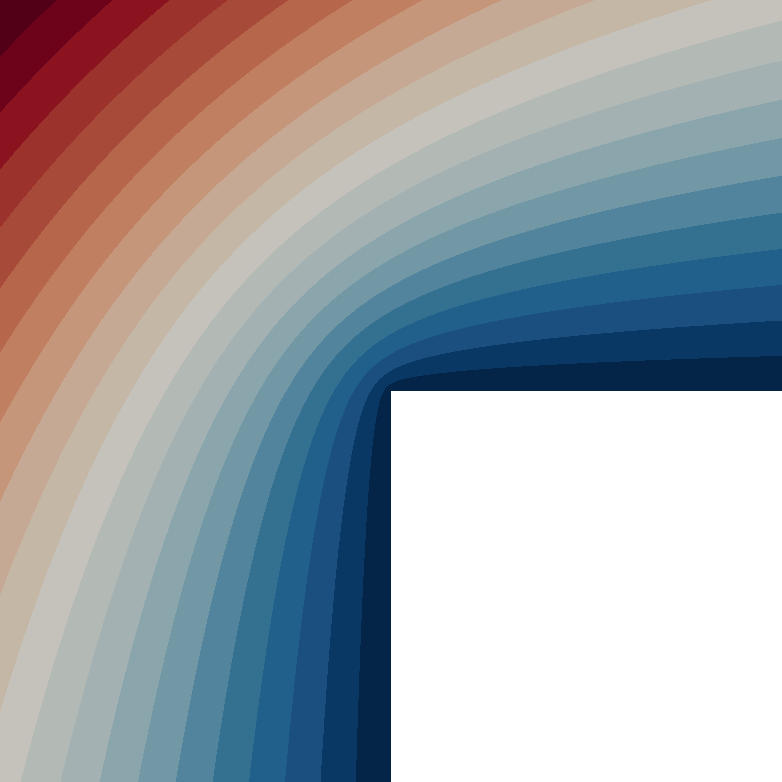
\includegraphics[width=0.49\textwidth]{solution}\hfill
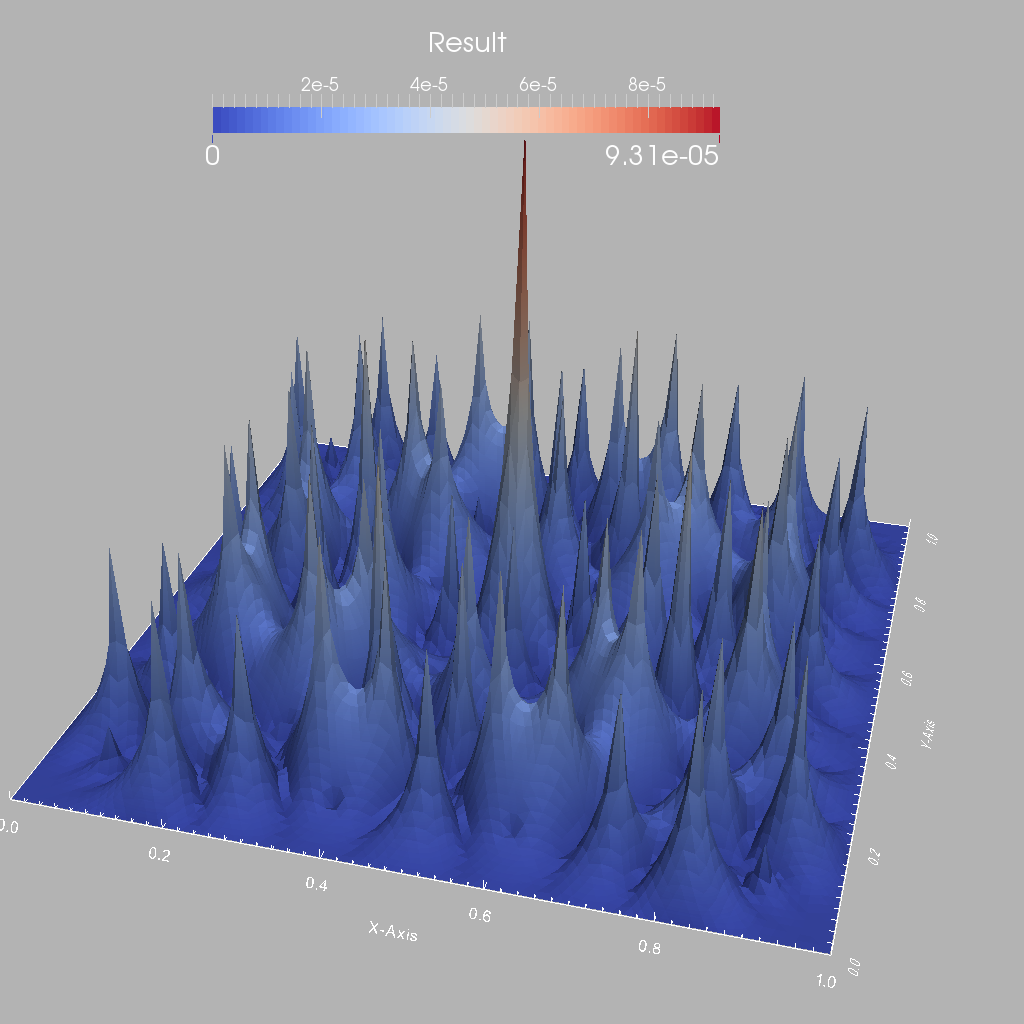
\includegraphics[width=0.49\textwidth]{error}
\end{center}
\caption{Finite element solution $u_h$ (left)
and absolute error $|u-u_h|$ (right) visualized as surface for a 
two-dimensional simulation.}
\label{fig:solution}
\end{figure}

\section{Outlook}

The interested reader can proceed in different directions from here.
The more obvious things are:
\begin{itemize}
\item Run the problem on various levels of refinement and determine
the maximum error. The maximum error should behave like $O(h^2)$
with the mesh size.
\item Try a different solution, like $u(x,y)=x^3+y^3$, change the program
accordingly and study the error with respect to mesh refinement.
\item Replace the algebraic multigrid preconditioner with a different one,
e.g. the BiCGStab method with SSOR preconditioner:
\begin{lstlisting}[basicstyle=\ttfamily\small,
frame=single,
backgroundcolor=\color{listingbg}]
  typedef Dune::PDELab::ISTLBackend_SEQ_BCGS_SSOR LS;
  LS ls(5000,true);
\end{lstlisting}
\end{itemize}
Other, more involved options which will be covered in further tutorials are:
\begin{itemize}
\item Implementation of Neumann type boundary conditions involving
boundary integrals.
\item Extension of the finite element method to cube elements using 
multi-linear basis functions.
\item Extension of the finite element method to higher order polynomials.
\end{itemize}

% bibtex bibliography
\bibliographystyle{plain}
\bibliography{tutorial00.bib}

\end{document}
